\section{Introduction}

Keys are used to encrypt high sensitive personal data and therefore
they must be kept safely.  Secure storage of private keys is known to
be a difficult problem --- especially for end-users with limited
skills in system administration and insufficiently redundant hardware.
A central objective for any solution is that only the legitimated
owner of a key must have the possibility to recover a lost key.

But how can one create a confidential backup of a key? It certainly
makes no sense to encrypt a key with a different password and then use
the result as a backup. After all, this merely shifts the problem from
the original key to the password, which is basically yet another key.
So simply encrypting the key is not helpful.  But without encryption,
any copy of a key increases availability, but also the risk of the
key's confidentiality being compromised.

Most people have difficulties memorizing a high-entropy
passphrase. Hence, existing key management ``solutions'' often reduce
the problem of memorizing one or more high-entropy passphrases or keys
to memorizing a single low-entropy passphrase. This is not a good
solution, as the low-entropy passphrase undermines security.

In this thesis, we describe a software solution for the described
problem using secret splitting.  We call our solution ``Anastasis'',
which is a medical term for the prognosis of full recovery.  We will
call the information that Anastasis allows the user to recover their
{\em core secret}.

\subsection{Principles}

For Anastasis we have following design objectives, in order of importance:

\begin{enumerate}
 \item Anastasis must be Free Software\footnote{\url{https://www.fsf.org/}}. Everyone must have the right to
   run the program, study the source code, make modifications and share
   their modifications with others.
 \item Anastasis must not rely on the trustworthiness of individual providers.
   It must be possible to use Anastasis safely, even if a subset of the
   providers is malicious. Anastasis must minimize the amount of information
   exposed to providers and the network.
 \item Anastasis must put the user in control: They get to decide which
   providers to use, and which combinations of authentication steps will
   be required to restore their core secret. The core secret always remains exclusively
   under the user's control, even during recovery.
 \item Anastasis must be economical viable to operate. This implies usability
   and efficiency of the system.
 \item Anastasis must support a diverse range of use cases.
\end{enumerate}


\subsection{Approach}

\subsubsection*{Secret sharing and recovery}

Our approach to solve the problem of key recovery is to let the user
split their core secret across multiple escrow providers (see
Figure~\ref{fig:system_arch2}). To recover their core secret, the user has to
authorize key the recovery, usually by passing an authentication check
which they configured for the respective provider.

After successful authentication the user receives the secret shares
and is able to reassemble their core secret locally on their computer.

\begin{figure}[H]
\centering
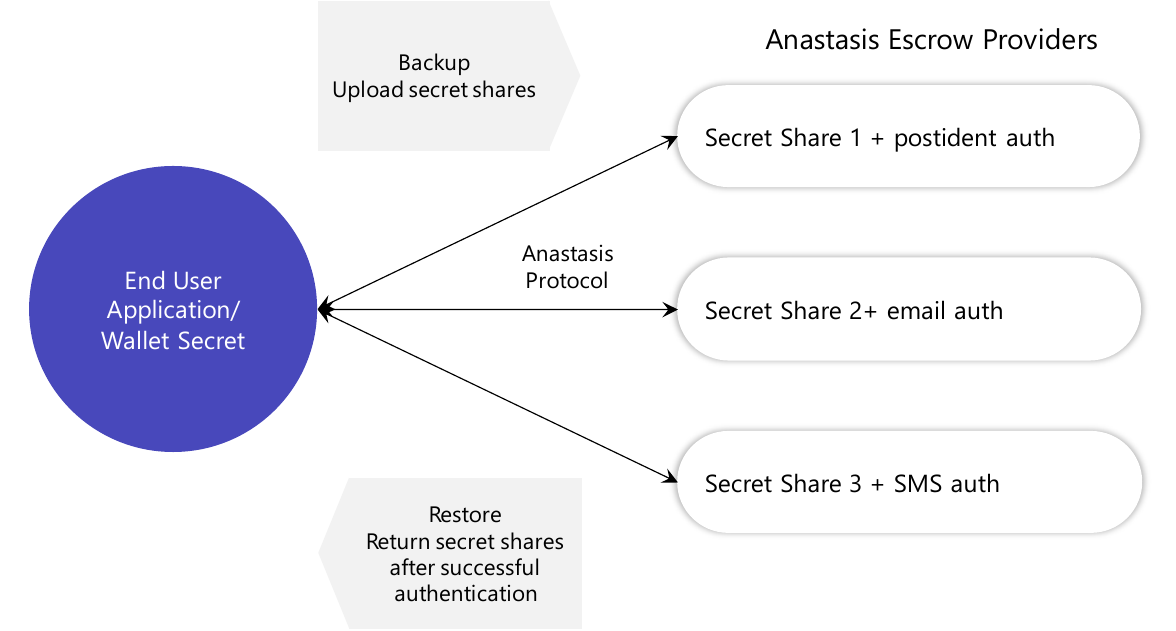
\includegraphics[scale=0.33]{images/system-architecture_2.png}
\caption{System architecture}
\label{fig:system_arch2}
\end{figure}

\subsubsection*{Derive user identifier}

Every person has some hard to guess, semi-private and unforgettable
inherent attributes such as name and passport number, social security
number or AHV~\cite{jerome2015} number (in Switzerland).  We use those attributes to
improve the security and privacy provided by Anastasis.  Basically,
these attributes serve as weak key material, raising the bar for
attackers without the availability disadvantages of passphrases ---
which users may forget.  Anastasis derives a ``user identifier'' from
such a set of unforgettable attributes (see Figure~\ref{fig:user_id}).

\begin{figure}[H]
\centering
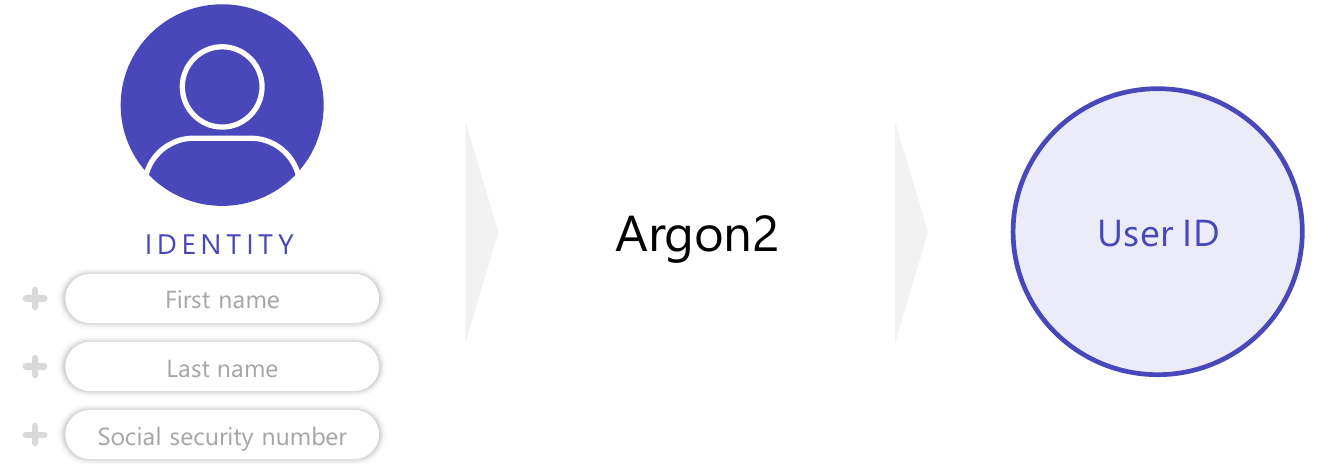
\includegraphics[scale=0.3]{images/user_id.png}
\caption{Derivation of a user identifier}
\label{fig:user_id}
\end{figure}

\subsubsection*{Encrypt and encrypt and encrypt}

Anastasis uses several layers of encryption. First, the user's core
secret is encrypted with a master key. The master key is encrypted
with various policy keys. The policy keys are derived from various
secrets which are encrypted and distributed across various providers
together with information about the desired recovery authorization
procedure. This last encryption is done based on keys derived from the
user identity.  These many layers of encryption are designed to
distribute trust and to minimize or delay information disclosure.

\subsubsection*{Private payments are integrated}

The Anastasis protocol includes provisions for privacy-preserving
electronic payments to the service providers, as well as resource
limitations to protect service providers against resource exhaustion
attacks.  This ensures that it should be possible to operate the
service commercially.


\subsection{Use cases}

There are several applications which are in need of a key escrow
system like Anastasis. Some of them shall be introduced in this
section.

\subsubsection{Encrypted email communication}

For email encryption using Pretty Good Privacy
(PGP)~\cite{garfinkel1995} users need a private key which is typically
stored on the device running PGP.  PGP uses a ``Web of trust'' to
establish the authenticity of keys.

Pretty Easy privacy (short p\equiv p) is ``a cyber security solution
which protects the confidentiality and reliability of communications
for citizens, for public offices and for
enterprises''~\cite{pepdoc}. It secures communication via email by
providing end-to-end encryption similar to PGP.  A major difference is
that p\equiv p uses opportunistic encryption and so-called trustwords
to establish authenticity to avoid usability and privacy problems
associated with the ``Web of trust''~\cite{caronni2000}.

The impact of losing control over the private key is similar in both
systems:

\begin{itemize}
  \item If the private key becomes unavailable, all emails which were
encrypted to that key become unreadable. Furthermore, the user would
likely need to rebuild their ``Web of trust''.
  \item If the private key is
disclosed to an adversary, they might be able to decrypt that user's
encrypted emails -- which may go back years and could include highly
sensitive information.  An adversary could also use the private key
to send cryptographically signed emails pretending to be the user.
\end{itemize}


\subsubsection{Digital currencies and payment solutions}

Another application relying on a core secret are cryptocurrencies like
Bitcoin. Each user of Bitcoin needs an electronic wallet which stores
and protects the private keys of the user. Those private keys
legitimate its owners to spend the bitcoins corresponding to the
keys.~\cite{LLLW*2017}

Losing Bitcoin wallet keys means losing all of the corresponding
Bitcoins.  The reader may be familiar with stories from the mass media
about people who claim to have lost their key to their electronic
wallet and therefore huge sums of
cryptocurrency~\cite{millions_lost}. Backup systems are essential to
avoid such cases.

The following graphic illustrates the keys used in Bitcoin
wallets. In this case, the core secret Anastasis would store
is the ``master key'' $m$:

\begin{figure}[H]
	\centering
	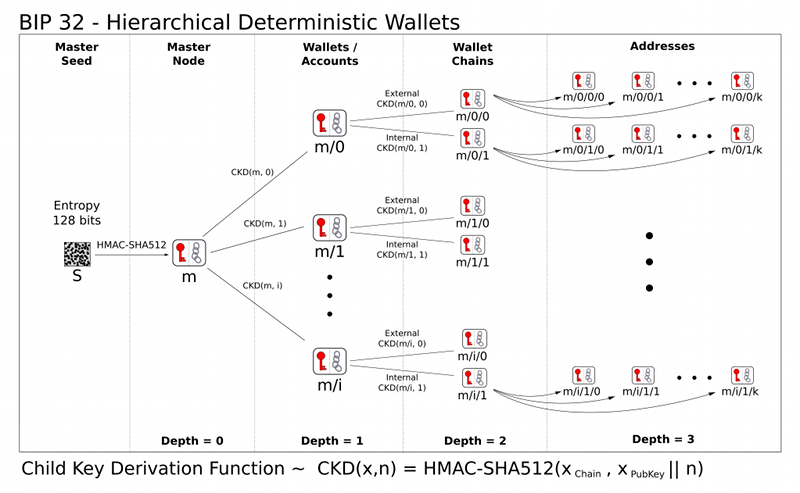
\includegraphics[scale=3.5]{images/bitcoin-keys.png}
	\caption[Master key in Bitcoin wallets]{Master key in Bitcoin wallets (from~\cite{bitcoin-keys})}
	\label{fig:bitcoin_keys}
\end{figure}

GNU Taler\footnote{\url{https://taler.net/de/}} is a new electronic instant payment system for
privacy-friendly online transactions. The GNU Taler digital wallets are
storing electronic coins, and backups are protected with a key.
Losing the backup key means losing all the money stored in the wallet,
as well as the transaction history kept in the wallet.

The European Central Bank (ECB) informally informed Taler Systems SA
about the requirement for electronic wallets denominated in Euros to
support password-less data recovery to ensure users would not loose
their electronic funds if their device were to be damaged or lost.

This was the key impulse which motivated us to create Anastasis,
with the goal of enabling recovery of GNU Taler's backup keys via
Anastasis.


\subsubsection{Password managers}

To avoid using low-entropy passwords and password reuse, some people
use software password managers like
KeePass\footnote{\url{https://keepass.info/}}. Such password managers
relieve you of the burden of remembering many passwords and in most
cases allow the generation of high-entropy passwords.

The user only has to remember the password for the password
manager. However, as discussed before, this is still a major problem:
\begin{itemize}
  \item On the one hand, users could use an insecure, easy to
remember password. In this case, an adversary gaining control
over the password manager's database could break into all systems
secured by keys managed by the password manager.
\item On the other hand, users could use a complex, high-entropy
  passphrase.  However, if that passphrase is forgotten, users
  face the loss of all passwords and thus also all online
  services that the password manager controlled for them.
\end{itemize}

Anastasis can be used to enable recovery of strong passphrases,
such as those that should be used to secure password managers.


\subsubsection{Hard drive encryption}

Data at rest is often protected using (full) drive encryption, for
example using software like
LUKS\footnote{\url{https://guardianproject.info/archive/luks/}}.  For
encryption and decryption of the drive a combination of key files,
passphrases and Trusted Platform Modules (TPMs)~\cite{bajikar2002} are
used.

Anastasis can be used to backup and restore such key files or
passphrases.
